\documentclass[10pt, conference, letterpaper]{IEEEtran}
\usepackage{cite}
\usepackage{xcolor,soul,framed}
\usepackage{amsmath,amsthm,amssymb,amsfonts}
\usepackage{algorithmic}
\usepackage{graphicx}
\usepackage{color, soul}
\usepackage{algorithm, algorithmic}
\usepackage[utf8]{inputenc}
\usepackage[english]{babel}
\usepackage{mathtools}
\graphicspath{ {./images/} }

%---------------------------------------------------------------%
\newtheorem{definition}{Definition}
\newtheorem{assumption}{Assumption}
\newtheorem{problem}{Problem}
\newtheorem{lemma}{Lemma}
\newtheorem{remark}{Remark}
\newtheorem{theorem}{Theorem}
\newtheorem{corollary}{Corollary}
\newtheorem{example}{Example}
\newcommand{\eq}{=}
\newcommand{\domZ}{\mathbb{Z}_{*}}
\newcommand{\vecOne}{\mathbf{1}}
\newcommand{\ind}{\mathbf{I}}
\newcommand{\mat}{\mathbf}
\newcommand{\Mult}{\text{Mult}}
\newcommand{\define}{\triangleq}
\newcommand{\leadto}{\Rightarrow}
\newcommand{\vecG}{\boldsymbol}
\renewcommand{\vec}{\mathbf}
\DeclarePairedDelimiter{\set}{\{}{\}}
\DeclarePairedDelimiter{\norm}{|}{|}
\DeclarePairedDelimiter{\Inorm}{\|}{\|_1}
\DeclarePairedDelimiter{\Paren}{\bigg(}{\bigg)}
\DeclarePairedDelimiter{\Bracket}{\bigg[}{\bigg]}
\DeclarePairedDelimiter{\Brace}{\bigg\{}{\bigg\}}
%---------------------------------------------------------------%
\newcommand{\apSet}{\mathcal{K}}
\newcommand{\esSet}{\mathcal{M}}
\newcommand{\jSpace}{\mathcal{J}}
\newcommand{\wSet}{\mathcal{W}}
\newcommand{\uSet}{\mathcal{U}}
\newcommand{\cSet}{\mathcal{C}}
\newcommand{\Stat}{\mathbf{S}}
\newcommand{\Obsv}{\mathcal{Y}}
\newcommand{\Policy}{\boldsymbol{\Omega}}
\newcommand{\BPolicy}{\bar{\Policy}}
\newcommand{\ASpace}{\mathbf{A}}
%---------------------------------------------------------------%

\begin{document}
    %=============================== TITLE ===============================%
    \title{
        Obsolete Partial Information-based Distributed Online Job Dispatching in Edge Computing System
    }
    % \author{
    %     \IEEEauthorblockN{
    %         Yuncong Hong\IEEEauthorrefmark{1}\IEEEauthorrefmark{2},
    %         Zhenhua Han\IEEEauthorrefmark{2}
    %         Rui Wang\IEEEauthorrefmark{1},
    %         Haisheng Tan\IEEEauthorrefmark{3},
    %         Francis C.M. Lau\IEEEauthorrefmark{2}
    %     }
    %     \IEEEauthorblockA{
    %         \IEEEauthorrefmark{1}Southern University of Science and Technology, P.R. China,
    %         \IEEEauthorrefmark{2}The University of Hong Kong, Hong Kong,\\
    %         \IEEEauthorrefmark{3}University of Science and Technology of China, P.R. China
    %     }
    % }
    \maketitle

    %============================== ABSTRACT ==============================%
    \begin{abstract}
        \label{sec:abstract}
        Edge computing is believed to be the solid solution for time-sensitive big data real-time calculation. The cooperation among edge servers in the system usually causes in-effective task scheduling due to obsolete information sharing which is hard to tackle.
        In this work, we formulate the problem with job dispatching in distributed Edge Computing system, and identify the difficulty exists in cooperation among AP nodes (Access Points) and ES nodes (Edge Servers) with delayed information. We design the broadcast information sharing scheme in the system and formulate the corresponding problem into a MDP problem. The value function approximation and one-step policy iteration method is adopted to obtain a sub-optimal dispatching policy whose performance can be bounded analytically.
    \end{abstract}

    % \begin{IEEEkeywords}
    %     Edge Computing, Job Dispatch, Delayed Information, Collective Observability, Distributed Multi-agent MDP
    % \end{IEEEkeywords}

    %============================ INTRODUCTION ============================%
    \begin{section}{INTRODUCTION}
        \label{sec:introduction}
        Edge Computation is believed to be a promising technology for solving increasingly communication congestion in backbone network.
        (Rich-media tasks are delay-sensitive).
        \cite{Naha2018} is a survey about fog computing in latency-aware computing in IoT, and investigate numerous proposed computing architecture.

        Related works on job dispatching on scheduling in edge computing, mostly with centralized agent to apply action and seldom take delayed information impact into consideration.
        There are some previous works on jobs scheduling strategies under the scenario of edge computation, together with joint optimization job dispatching and resource allocation:
        \begin{itemize}
            \item \cite{Zheng2019} is a work considering maximizing the long-term utility in MEC offloading policy, and formulating the problem with MDP solved with Q-learning (However, it's applied with a centralized controller which would suffer from communication overhead, and the proposed reduced states is naive);
            \item \cite{Du2018} propose an offline algorithm with MINLP (Mixed-Integer Nonlinear Programming) problem formulation, considering min-max fairness guarantee in computation offloading and computation resource allocation in fog/edge computing scenario (However, with only one edge and one cloud node considered);
            \item \cite{Alameddine2019} is a work considering task offloading, scheduling and resource allocation joint optimization with Benders Decomposition (However, delay information is previous defined);
            \item \cite{Fan2017} considers cooperation of multiple MEC-BSs of computation offloading to other MEC-BSs (However, it doesn't consider the offloading utility impact on other MEC-BSs, i.e. only optimize for one BSs in the cluster).
        \end{itemize}
        
        Different from the previous referred works, which only consider optimization for one agent in system or using centralized agent for decision making, we focus on the impact of out-of-dated information on decision making in multiple agents distributed cooperation.
        Due to frequent jobs releasing from users and uncertainty of jobs uploading time to servers, the obsolete information is inevitable in a purely distributed system.
        This information sharing delay would cause severe misestimate for job dispatching decision making, and thus it will be hard to guarantee the cooperation among individual agents.
        Moreover, the information sharing delay is often un-deterministic due to shared underlaid network topology, and offensively sharing strategy would cause network congestion to other normal functions.

        As what we have learned for now, there are very limited discussions on this topic:
        \begin{itemize}
            \item The earliest works entangling with out-of-dated information we could find is \cite{ref-01} (cited 167 times). In this work, the single agent is assumed not able to observe the global state, and thus they need communication to establish cooperation by sharing limited information. The agent considers communication as extra action to synchronize the states and thus incurs extra cost (However, the communication is without delay, thus converted into POMDP problem);
            \item The other work \cite{ref-02} considers continuous state observation with constant or stochastic delay with single agent;
            \item One researcher published a series of paper on this topic \cite{Lyu2017,Lyu2018,Lyu2018a,Lyu2018b}.
                \cite{Lyu2017} is work considering \emph{out-of-date knowledge} optimization in IoT computing scenario, with Lyapunov optimization;
                \text{[delay-sensitive, ToC]} \cite{Lyu2018} identify that task admission is critical to delay-sensitive applications in mobile edge computing, and proposes an (1-$\epsilon$)-approximation algorithm
                \text{[foggy, fully distributed online]} \cite{Lyu2018a} is a work fully distributed online optimization to minimize the time-average cost and achieve asymptotic optimality over infinite time;
                \cite{Lyu2018b} try to establish cooperation among selfish devices in fog computing, and out-of-date information is blamed for optimality gap but proved to asymptotically diminish with the proposed algorithm (However, the out-dated information is considered with limited effect);
        \end{itemize}

        % Service Placement Scenario:
        % \begin{itemize}
        %     \item \cite{Rodrigues2017} is a work on minimizing service delay in mobile edge computing;
        %     \item \cite{Yang2016} is a work considering services placement and requests dispatching on edge servers, and leverage users' pattern to predict "service cache" for online decision making;
        %     \item \cite{Chen2018} is a work with SDN on task offloading and battery life saving, and solve the NLP problem with two sub-problems;
        % \end{itemize}
        % Using Game Theory:
        % \begin{itemize}
        %     \item \cite{yang2018} and \cite{Josilo2019a} considers distributed computation offloading game;
        %     \item \cite{Liu2018} is a work considering minimize users' power consumption with Lyapunov optimization and matching theory;
        %     \item \cite{Dinh2018} considers distributed multi-user offloading in wireless channel with selfish EPG (exact potential game);
        %     \item \cite{Josilo2019} considers selfish offloading to achieve Nash equilibrium;
        %     \item \cite{Chen2016} is a work considering multi-user computation offloading with multi-channel contention, and adopt game theory approach to achieve Nash equilibrium with upper bound of convergence time;
        %     \item \cite{Zhang2018} considers multi-user offloading under transmit power decision and user association decision;
        % \end{itemize}
        % System Work:
        % \begin{itemize}
        %     \item \cite{Yu2018} is a system work published in ToMC, presents a framework to minimize remote execution overhead, and carry out real system experiments using large-scale data from cellular network provider;
        %     \item \cite{Wang2018} is a system work published in IEEE Access, considers the mobility of mobile users in limited coverage solved with service migration and handover, and propose a framework;
        % \end{itemize}

        In this article, we consider there are Access Points (AP) in this network to connect the User Equipment (UE) and the Edge Servers (ES).
        The computation jobs would be released from UEs and the dispatching decisions are determined distributed on each APs as depicted in Fig.\ref{fig:system}.
        The information sharing scheme is proposed in this article with synchronized broadcast design. With the help of this scheme, we could immediately apply the job dispatching decision based on obsolete information, with some prior stochastic knowledge of global system.
        Our contributions are summarized as follows.
        \begin{itemize}
            \item To our best knowledge, we are the first work to propose the MDP framework making use of obsolete information in edge computing system. With shared prior stochastic knowledge, the distributed agent could come to consensus on optimal oplicy adopting globally;
            \item We propose a global state MDP formulation to characterize the multi-agent problem, i.e. single agent would consider multi-agent decision optimality to achieve cooperation.
            We with adopt value function approximation to reduce the traditional algorithm complexity, and come up with performance guarantee performance bound.
        \end{itemize}

        \hl{The remainder of this paper is organized as follows.}
        In Sec.II, system model.
        In Sec.III, problem formulation.
        In Sec.IV, we introduce low-complexity MDP algorithm.
        In Sec.V, evaluation.
        In Sec.VI, conclusion.
    \end{section}

    %============================ SYSTEM MODEL ============================%
    \begin{section}{SYSTEM MODEL}
        \label{sec:model}
        \begin{subsection}{Network Model}
            We have Access Points (AP) and Edge Servers (ES) denoted as $\apSet \define \set{1,\dots,K}$ and $\mathcal{M} \define \set{1,\dots,M}$ respectively in our MEC (mobile edge computing) system depicted in Fig. \ref{fig:system}. In this system, we adopt the same timing mechanism at both AP and ES side with a minimum \emph{timeslot} lasting for $\tau$ seconds.

            \begin{figure}[ht]
                \centering
                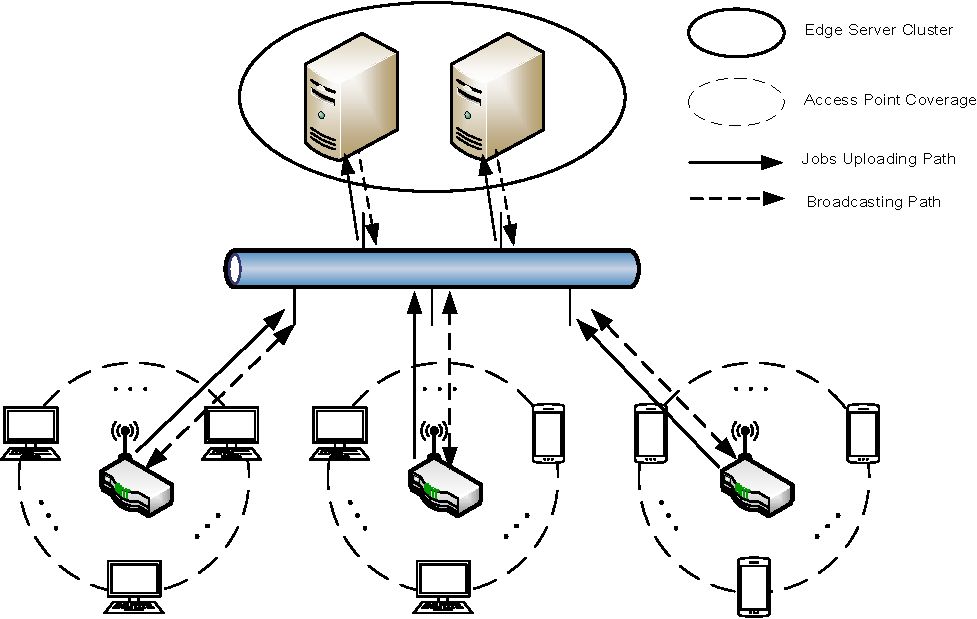
\includegraphics[width=0.45\textwidth, trim={0.5cm 0.5cm 0.5cm 0.5cm}, clip]{system-model.pdf}
                \caption{The Illustration of MEC System Model}
                \label{fig:system}
            \end{figure}

            The User Equipment (UE) would offload the computation jobs on demand to the AP it connect.
            We consider some types of jobs are supported on edge servers with Virtual Machine (VM) resources. The job space is denoted as $\jSpace \define \set{1,\dots, J}$, and jobs type distribution on each AP node follows the same distribution over $\jSpace$.
            % which is obtained by statistics and denoted as $p_j \define \Pr\{\text{"j-type arrival"}\}$, where $\sum_{j\in\jSpace} p_j=1$.
            Thus the job arrival process on $k$-th AP ($\forall k\in\apSet$) is compounded of the job arrivals from all UEs connected, which follows the assumption as:
            \begin{assumption}[Job Arrival Process for AP]
                The $j$-type job arrival distribution for $k$-th AP is denoted as $A_{k,j}$, which is independent and identically distributed (i.i.d) over each timeslot as $A_{k,j} \sim Bernoulli(\lambda_{k,j})$, $\lambda_{k,j}\in[0,1]$. This implies that there will be at most one $j$-type job arrives on $k$-th AP in one timeslot. According to \emph{Poisson Limit Theorem}, the arrival process is a memory-less exponential process with average arrival rate $\mathbb{E}[A_{k,j}]=\lambda_{k,j}$.
            \end{assumption}

            The AP itself is assumed with no computation capability, and thus it need to further dispatch those jobs to the edge servers.
            The jobs arrival in each timeslot on AP will be immediately dispatched to edge servers.
            {\color{red}The corresponding uploading delay of one job is stochastic and job-type independent over one AP-ES link, which is denoted as $U_{k,m}$ from $k$-th AP to $m$-th ES ($\forall k\in\apSet, \forall m\in\esSet$) and upper bounded by $\hat{U}_{k,m}$.
            And we have $\vec{U} \define \set{U_{k,m}|\forall k\in\apSet,m\in\esSet}$ to denote the set of distribution information about uploading delay. The expectation of link uploading time is denoted as $\bar{u}_{k,m}$.}

            After arrival on edge servers, the jobs will join computation queue with the supported VM.
            Each VM is considered running parallel without resource contention, and the jobs scheduling for each VM is with a single queue following \emph{FCFS} (First-Come-First-Serve).
            {\color{red}The maximum queue length is set to discourage too many jobs pending on edge servers and is denoted as $L_Q$. The job submission over the limit will be rejected and announce the AP where the job is from.}

            {\color{red}For jobs processing on edge servers, we adopt \emph{unrelated machines} assumption in \cite{tan-online}, where the job processing time on different servers are machine dependent and variant of resource or VM (virtual machine) constraints.
            Moreover, we have $l_{m,j}$ to denote the processing time for $j$-type job on $m$-th edge serer following some distribution, whose largest processing time is bounded by $l_C$.}

            For convenience, we assign type of jobs on edge servers which have no VM resource available with \emph{infinity} processing time, and this kind of dispatching possibility will be rejected at the AP side.
        \end{subsection}

        \begin{subsection}{Information-Sharing Broadcast Model}
            As there is no centralized agent to distribute dispatching decisions to each AP node, an efficient information sharing scheme is needed to help collect global information and establish cooperation among standalone nodes.
            In this paper, the proposed sharing scheme is designed via periodic broadcasting, where all the AP and ES nodes in the system should broadcast their system related information with a same period interval as $t_B$. More specifically, the broadcasting is applied in a synchronized way that all the nodes start to broadcast at the start of same timeslot and repeat broadcasting after the same periodic interval $t_B$. We call each periodic point of broadcasting as \emph{broadcast point} and denote the $i$-th broadcast with $t_i$ where,
            \begin{align}
                t_i = i \cdot t_B, i=0,1,2,\dots
            \end{align}
            For $i$-th \emph{broadcast point}, the composed broadcast information from all the AP and ES nodes, and the corresponding information is listed as follows.
            \begin{itemize}
                \item The $k$-th AP ($\forall k\in\apSet$) contains information $\mat{R}_k(i) \define (r^{(k)}_{m,j}(i))_{\set{m\in\esSet,j\in\jSpace}}$, where $r^{(k)}_{m,j}(i)$ denotes the remaining number of $j$-type jobs in uploading to $m$-th ES at time $t_i$; and we have $\vec{r}^{(k)}_{m} \define (r^{(k)}_{m,j}(i))_{j\in\jSpace}$ to denote the rows in $\vec{R}_k(i)$; % and $\vec{\hat{r}}^{(k)}_{j}$ to denote the columns;
                \item The $m$-th ES ($\forall m\in\esSet$) contains information $\vec{Q}_m(i) \define \set{Q_{m,j}(i)|\forall j\in\jSpace}$ to denote the computation queues for different job types, where $Q_{m,j}(i) \define (n_{m,j}(i), \delta_{m,j}(i))$ to characterize the $j$-type FIFO queue on $m$-th ES; $n_{m,j}(i)$ denotes the number of $j$-type job queueing on $m$-th ES, and $\delta_{m,j}(i)$ denotes the remaining processing time for last job.
            \end{itemize}
            Thus the composed broadcasting information is denoted as:
            \begin{align}
                \Obsv_i \define
                        \Brace{
                            \set{\mat{R}_{k}(i)|\forall k\in\apSet},
                            \set{\vec{Q}_m(i)|\forall m\in\esSet}
                        },
            \end{align}
            where $\Obsv_i$ is a set of global information of $i$-th broadcast. And it's actually the global system states at $t_i$.

            {\color{red}Due to the shared underlaid network with other network functions, the broadcast latency is \emph{un-predictable} in a distributed system and each AP will have different delay when receiving all the broadcast information from all the ES nodes and other AP nodes.}
            Let $D^{(p)}_{k,k'}$ denotes the broadcast delay between two AP nodes from $k'$-th AP to $k$-th AP ($\forall k,k'\in\apSet$); let $D^{(s)}_{k,m}$ denotes the broadcast delay between AP and ES node from $m$-th ES to $k$-th AP ($\forall k\in\apSet,\forall m\in\esSet$).
            Furthermore, we denote the latency for $k$-th AP receives broadcast information from other nodes (including all ES nodes and other AP nodes) as \emph{Update Latency}. There are total $(K+M)$ latency time points for one AP and especially, the latency time from itself to itself is always zero. Without loss of generality we give the definition for update latency listed in the order from smallest to largest as follows.
            \begin{definition}[Update Latency]
                For $k$-th AP ($\forall k\in\apSet$), every latency time points for receiving other nodes' broadcast with respect to latest broadcast point are listed as follows.
                \begin{align}
                    D_{k,0}, D_{k,1}, \dots D_{k,N'},
                \end{align}
                where $N'\define(K+M-1)$, and $D_{k,0}\equiv0$ to denote the broadcast information latency generated on itself. Due to the unpredictable property of broadcast latency, there is no explicit mapping between the second sub-script with indexes of $\apSet$ or $\esSet$ (except for $0$). And we could not explicitly denote the information update at each time point for $k$-th AP.
            \end{definition}
            {\color{red}Furthermore, We assume that broadcast latency $D_{k,n}$ is bounded with $[0, \hat{D}_{k,n}]$ and follows some distribution in this interval summarized from statistical data, which is denoted as $\eta_{k,n}(d) \define \Pr\{D_{k,n}=d\}$ with mean as $\bar{d}_{k,n}$ ($\forall k\in\apSet,\forall n\in\set{1,\dots,N'}$).
            And we have $\vecG{\eta} \define \set{\eta_{k,n}|\forall k\in\apSet,n\in\set{1,\dots,N'}}$ to denote the latency distribution set for all AP nodes.}

            The broadcast design introduces a \emph{Two-time scale} structure in the MEC system.
            The job dispatching and scheduling decisions on AP and ES side respectively are still carried out based on timeslot scale, while the policy update is based on broadcast interval with the information update.
            More specifically, the AP would change its policy when receives partial information and update its policy when it receives all the broadcast information which implies that it comes to consensus on the obsolete global information with other AP nodes.
            {\color{red}The multi-stage policy promises that the AP agent is aware of  Moreover, we implement the broadcast in a low-frequency way that the broadcast period is always larger than the maximum broadcast latency pulsing the maximum uploading delay, i.e. $t_B > \hat{D}_{k} + \hat{U}_{k,m}$ $(\forall k\in\apSet, \forall m\in\esSet)$.}

            Due to the broadcast latency, the information received with delay will affect the policy update point for each AP, which impact on the transition distribution of next-stage policy and global states.
            {\color{red}In the next section, we will show that with the prior statistic knowledge about broadcast latency $\vecG{\eta}$, we could establish exact cooperation among AP nodes under MDP frame work with analytical performance bound.}
        \end{subsection}
    \end{section}

    %============================ FORMULATION =============================%
    \begin{section}{PROBLEM FORMULATION}
        \label{sec:formulation}
        In this section, we formulate the standard MDP problem with respect to the broadcast-point time scale. The formulated problem is based on global information shared via synchronized broadcast, and the the optimal solution is achieved via compounded dispatching policies on all AP nodes.
        Given the fact that AP nodes would obtain global states update only after \emph{Update Latency} in each broadcast interval, the formulated MDP problem is composed of two adjacent broadcast interval with obsolete information and updated information.
        Then we show that the solution for all AP nodes suffers from curse of dimensionality and a low-complexity solution is needed.

        \begin{subsection}{System State and Dispatching Policy}
            The system states is selected based on the nature that $k$-th AP comes up with complete broadcast information only after its corresponding \emph{Update Latency} in the broadcast interval.
            The relative difference between broadcast point and the update time point is depicted in Fig. \ref{fig:br-trans} \hl{(need to modify the state denotation in figure)}.
            \begin{definition}[System State]
                The system state at $i$-th broadcast point is denoted as $\Stat_i \define (\Obsv_{i}, \Obsv_{i-1}), (i=1,2,\dots)$, where $\Obsv_{i-1}$ represents the obsolete information before the broadcast received, and $\Obsv_{i}$ represents the updated information after the corresponding $D_k$ delay for $k$-th AP node.
            \end{definition}

            \begin{figure}[ht]
                \centering
                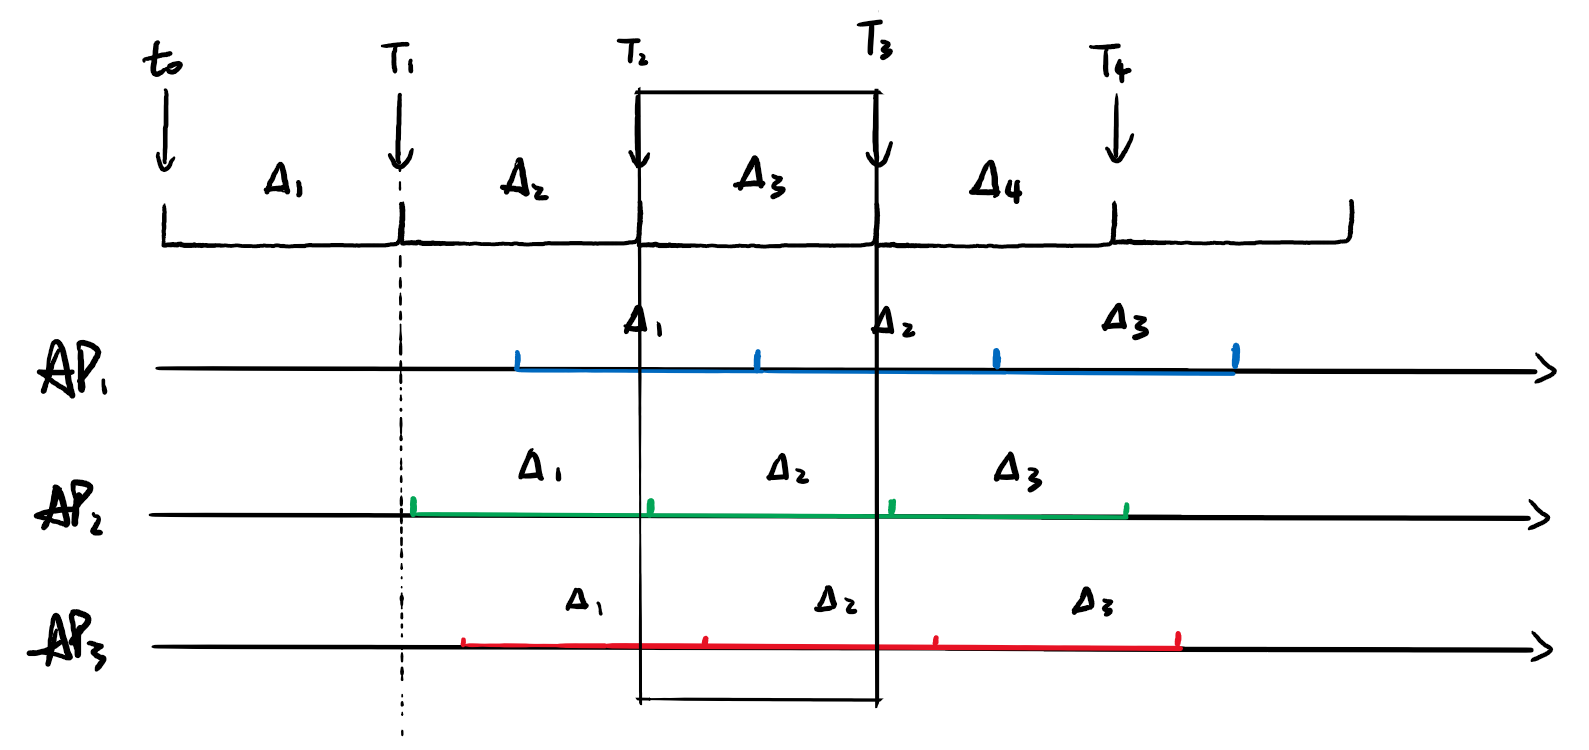
\includegraphics[width=0.45\textwidth]{broadcast-trans.png}
                \caption{Global Consensus and Transition with Delayed Action}
                \label{fig:br-trans}
            \end{figure}

            The \emph{dispatching policy} is applied over arrival jobs in each timeslot on each AP, and the \emph{dispatching action space} is defined as $\mathbf{A}: (j, m) \in \jSpace \times \esSet$, where $(j, m)$ denotes the action that $j$-type job should be uploaded to $m$-th ES.
            Based on the two stages of global system information $\Obsv_{i-1}$ and $\Obsv_{i}$ in system state, the compounded global-wise policy of all AP nodes is defined as follows.
            \begin{definition}[Compounded Dispatching Policy]
                The compounded dispatching policy over $\Stat_{i}$ is defined as $\Policy(\Stat_{i})$ which is composed of all the local policies $\Omega_k(\Stat_{i})$ ($\forall k\in\apSet$) as:
                \begin{align}
                    \vecG{\Omega}(\Stat_{i}) \define 
                    \Bracket{
                        \Omega_{1}(\Stat_i),
                        \dots,
                        \Omega_{K}(\Stat_i)
                    }.
                \end{align}
                More specifically, $\Omega_k(\Stat_{i})$ is composed of two-stage policy:
                \begin{align}
                    \Omega_k(\Stat_i) \define
                    \begin{bmatrix}
                        \tilde{\Omega}^{(0)}_k(\Obsv_{i-1}), \dots, \tilde{\Omega}^{(N')}_k(\Obsv_{i-1}),
                        \nonumber\\
                        \tilde{\Omega}^{(0)}_k(\Obsv_{i}), \dots, \tilde{\Omega}^{(N')}_k(\Obsv_{i})
                    \end{bmatrix},
                \end{align}
                where $\tilde{\Omega}^{(n)}_k(\Obsv_{i}) \define \set{\omega^{(i,n)}_{k,m}(j)|\forall j\in\jSpace, \forall m\in\esSet}$ ($\forall n\in\set{0,\dots,N'}$) and $\omega^{(i,n)}_{k,m}(j)$ denotes the stochastic dispatching policy that: after $k$-th AP receiving $n$-th broadcast information component of $\Obsv_{i}$, the probabilistic action that upload $j$-type job to $m$-th ES ($\sum_{j\in\jSpace} \Pr\{\omega^{(i,n)}_{k,m}(j)\}=1$).
            \end{definition}
            More specifically, the multiple phases of the policy $\Omega_k(\Stat_i)$ are separated by \emph{Update Latency} $D_{k,n}$ for $k$-th AP ($\forall n\in\set{0,\dots,N'}, k\in\apSet$). One vivid example of policy adaption phase is given as follows.
            \begin{example}[Policy Phase Adaption]
                In the time interval $[t_{i}, t_{i+1}]$, $k$-th AP would adopt $\tilde{\Omega}^{(0)}_k(\Obsv_{i-1})$ before $t_i$ and adopt $\tilde{\Omega}^{(1)}_k(\Obsv_{i-1})$ immediately at $t_i$ with its own information; then it will adopt $\tilde{\Omega}^{(n+1)}_k(\Obsv_{i-1})$ after receiving $n$-th broadcast information and adopt $\tilde{\Omega}^{(0)}_k(\Obsv_{i})$ immediately after receiving $N'$-th broadcast, i.e. the time when receiving all components of $\Obsv_{i}$.
            \end{example}
        \end{subsection}

        \begin{subsection}{The Optimization Problem}
            The optimization target of our problem is to minimize the \emph{average response time} of all jobs, which is composed of uploading time from AP to ES, and queueing-and-service time on ES nodes. According to \emph{Little's Law}, the average response time of all the jobs is equally as average number of jobs in system.

            Besides the cost counted for job response time, we furthermore add penalty on full-queue and empty-queue.
            The full-queue penalty is for the jobs submission would be rejected.
            {\color{red}The empty-queue penalty is given for the reason that the uploaded jobs in current broadcast interval will keep waiting on edge servers and to discourage the meaningless waiting time on edge servers, the edge servers will announce all the AP nodes the \emph{empty-queue-penalty} attached in next broadcast information.}

            Therefore, based on the system state definition, we have cost function as:
            \begin{align}
                &g\Paren{\Stat_{i}, \Policy(\Stat_{i-1})}
                \nonumber\\
                \define& \sum_{m\in\esSet}\sum_{j\in\jSpace} \Brace{
                        \alpha I[n_{m,j}(i)=0] + \beta I[n_{m,j}(i)=L_Q]
                    }
                    \nonumber\\
                    &+\sum_{k\in\apSet}\sum_{m\in\esSet} \Inorm{\vec{r}^{(k)}_{m}(i)} + \sum_{m\in\esSet}\sum_{j\in\jSpace} n_{m,j}(i),
            \end{align}
            where $\Inorm{\vec{r}^{(k)}_{m}}$ denotes the $L^1$-norm of vector $\vec{r}^{(k)}_{m}$, i.e. the sum up of absolute value of each entry; $\alpha$ and $\beta$ are weight factor for empty-queue penalty and full-queue penalty respectively.
            {\color{red}The cost function defined is a sampling of interval $t_B$ over the whole job response process, because the global information for AP nodes only contains the information at the broadcast points.}

            Our distributed optimization problem definition is given as follows.
            \begin{problem}[Distributed Cooperative Job Dispatching Problem]
                \begin{gather}
                    \min_{\Policy} \lim_{T \to \infty}
                        \mathbb{E}_{\Policy, \vecG{\eta}, \vec{U}}
                            \Bracket{\sum_{i=2}^{T} \gamma^{i-1} g(\Stat_{i}, \Policy(\Stat_{i-1}))|\Stat_1},
                \end{gather}
                where the cost is collected with a discount factor $\gamma$, and $\Policy$ denotes the global compounded policy of all AP nodes.
            \end{problem}

            According to \cite{sutton1998introduction}, the above problem could be solved by the following \emph{Bellman's equation}:
            \begin{align}
                V(\Stat_i) =& g(\Stat_i) +
                    \gamma \min_{\Policy(\Stat_{i})} \sum_{\Stat_{i+1}} \sum_{k\in\apSet}\sum_{d_k\in[0,\hat{D}_k]} \eta_k(d_k) \cdot
                    \nonumber\\
                    &\Pr\{ \Stat_{i+1}|\Stat_{i}, \Policy(\Stat_{i}) \} V(\Stat_{i+1})
                \nonumber\\
                =& g(\Stat_i) + \gamma \min_{\BPolicy(\Stat_{i})} \sum_{\Stat_{i+1}}
                \Pr\{ \Stat_{i+1}|\Stat_{i}, \BPolicy(\Stat_{i}) \} V(\Stat_{i+1}),
            \end{align}
            {\color{red}where $\BPolicy(\Stat_{i}) \define [\bar{\Omega}_1(\Stat_{i}), \dots, \bar{\Omega}_K(\Stat_{i})]$; each $\bar{\Omega}_k(\Stat_{i})$ on $k$-th AP denotes the policy phase separated by $\bar{d}_k$.}
            The definition for value function is defined according to the form in \cite{sutton1998introduction} as follows.
            \begin{align}
                V(\Stat_{i}) \define \lim_{T\to\infty}
                    \mathbb{E}_{\Policy,\vecG{\eta}} \Bracket{
                        \sum_{l=0}^{T} \gamma^l g\Paren{\Stat_{i+l}, \Policy(\Stat_{i+l-1})}
                    }.
            \end{align}

            % Before diving into the analysis on the transition function expression, we firstly come up with some probability denotations for arrival process on edge servers.
            % The job arrival processes for AP nodes under dispatching policy compose the job arrival process for ES nodes, which could be expressed as compounded of \emph{numbers arrival distribution} and \emph{processing time distribution} for $j$-type job ($\forall j\in\jSpace$).
            % \begin{itemize}
            %     \item The \emph{numbers arrival distribution} on $m$-th ES is composed of i.i.d Bernoulli distribution in each timeslot from independent AP nodes. The PMF (probability mass function) of the Bernoulli distribution from $k$-th AP under policy $\Omega_k(i)$ is denoted as:
            %     \begin{align}
            %         p_{k,m}^{(i)}(j) \define& \lambda_k p_j \cdot
            %             \frac{
            %                     \Pr\{\omega_{k,m}^{(i)}(j)\}
            %                 }{
            %                     \sum_{j\in\jSpace} \Pr\{\omega_{k,m}^{(i)}(j)\}
            %                 },
            %     %     \\
            %     %     p_{k,m}^{(i)} \define& \sum_{j\in\jSpace} p_{k,m}^{(i)}(j),
            %     \end{align}
            %     and we have $\rho_{k,m}^{(\Pi_k)}$ denotes the distribution under time-invariant policy $\Pi_k$ for $k$-th AP;
            %     \item The \emph{processing time distribution} is job-independent, thus the processing time on different edge servers keeps its original distribution and is determined when the time it joins the processing queue.
            % \end{itemize}
            
            \begin{lemma}[Transition Function Decoupling]
                The transition function in Bellman's equation could be decoupled on AP nodes states and ES nodes states, which will facilitate the approximated value function expression in the following section. The decoupled transition function is in the form as follows.
                \begin{align}
                    & \Pr\{\Stat_{i+1}|\Stat_{i}, \BPolicy(\Stat_{i})\}
                    \nonumber\\
                    =& \prod_{k\in\apSet} \Pr\Brace{\vec{R}_k(i+1)|\BPolicy(\Stat_{i})} \times \prod_{m\in\esSet}\prod_{j\in\jSpace}
                        \nonumber\\
                        & \Pr \Brace{Q_{m,j}(i+1)|Q_{m,j}(i), \set{\vec{R}_k(i)|\forall k\in\apSet}, \BPolicy(\Stat_{i})},
                \end{align}
                where first production part denotes the unfinished uploading state transition for AP nodes whose distribution, and the second part denotes the queueing state transition for ES nodes.
            \end{lemma}
            \begin{proof}
                Please refer to appendix \ref{trans-decouple}.
            \end{proof}

            As the formulated problem above is of infinite states and the action space would be exponentially expanded with respect to number AP and ES nodes, we could not use traditional \emph{policy iteration} or \emph{value iteration} algorithm \cite{sutton1998introduction} for unacceptable computational complexity. To alleviate curse of dimensionality, we take baseline dispatching policy to approximate the value function for each AP and ES nodes, and then carry out one-step iteration to obtain a better value function approximation.
        \end{subsection}
    \end{section}

    %============================= ALGORITHM ==============================%
    \begin{section}{LOW-COMPLEXITY SOLUTION}
        \label{sec:algorithm}
        In this section, we introduce a heuristic dispatching algorithm as the baseline policy, whose value function could be derived analytically. Then the joint expression with transition function as the optimization problem on right-hand side, we could further reduce the state complexity with averaged queueing dynamics on ES nodes.
        \hl{The proposed low-complexity sub-optimal policy can be obtained via the above approximated value function and one-step policy iteration. The derived value function becomes the cost upper bound of the proposed policy.}

        \begin{subsection}{Baseline Dispatching Policy}
            The baseline dispatching policy is adopted to obtain an approximation of value function. The policy on each AP nodes is randomized and time-invariant which is denoted as:
            \begin{align}
                \vec{\Pi} \define \Bracket{\Pi_1, \Pi_2, \dots, \Pi_K},
            \end{align}
            where $\Pi_k \define \set{\omega_{k,m}(j)|\forall m\in\esSet,\forall j\in\jSpace}$, $\forall k\in\apSet$.

            According to the additive structure of cost function, the value function could be divided linearly into two section as $\tilde{W}^{(p)}(\Obsv^{(p)}(i))$ and $\tilde{W}^{(s)}(\Obsv(i))$ under baseline policy:
            \begin{align}
                V(\Stat_{i}) =& 
                    g(\Stat_{i}) + \gamma \min_{\BPolicy(\Stat_{i})} \sum_{\Stat_{i+1}} \Pr\{ \Stat_{i+1}|\Stat_{i}, \BPolicy(\Stat_{i}) \}
                    \nonumber\\
                    & \cdot \Bracket{ \tilde{W}^{(p)}\Paren{\Obsv^{(p)}(i+1)} + \tilde{W}^{(s)}\Paren{\Obsv(i+1)} },
            \end{align}
            where $\tilde{W}^{(p)}(\cdot)$ and $\tilde{W}^{(s)}(\cdot)$ denote the split value function over AP nodes and ES nodes respectively; $\Obsv^{(p)}(i) \define \set{\mat{R}_k(i)|\forall k\in\apSet}$ and $\Obsv^{(s)}(i) \define \set{\vec{Q}_m(i)|\forall m\in\esSet}$ respectively denote the AP states collection and ES states collection for $\Obsv(i) = \set{\Obsv^{(p)}(i), \Obsv^{(s)}(i)}$, and the split value function is in the following form:
            \begin{align}
                &\tilde{W}^{(p)}\Paren{\Obsv^{(p)}(i)} \define \sum_{k\in\apSet}\sum_{m\in\esSet}
                    \mathbb{E}_{\Pi}\Bracket{\sum_{l=0}^{\infty} \gamma^{l} \Inorm{\vec{r}^{(k)}_{m}(i+l)}}
                \\
                &\tilde{W}^{(s)}\Paren{\Obsv(i)} \define \sum_{m\in\esSet} \sum_{j\in\jSpace}
                    \mathbb{E}_{\Pi}\Bracket{\sum_{l=0}^{\infty} \gamma^{l} n_{m,j}(i+l)}
            \end{align}
            The decoupled value functions for AP and ES nodes is obtained with an approximated form under the baseline policy.

            The approximated value function $\tilde{W}^{(p)}(\Obsv^{(p)}(i+1))$ for AP nodes is obtained as:
            \begin{align}
                \tilde{W}^{(p)}(\Obsv^{(p)}(i+1)) = \frac{1}{1-\gamma}
                    \sum_{k\in\apSet}\sum_{m\in\esSet} \mathbb{E}_{\Pi}[\Inorm{\vec{r}^{(k)}_{m}}],
            \end{align}
            where the expectation of $\Inorm{\vec{r}^{(k)}_{m}}$ under the policy $\Pi_k$ is actually a constant as expectation of Binomial distribution $\mathbb{E}_{\Pi_k}[\Inorm{\vec{r}^{(k)}_{m}}] = \sum_{j\in\jSpace} u_{k,m} \rho^{(\Pi_k)}_{k,m}(j)$.
            
            The approximated value function $\tilde{W}^{(s)}(\Obsv(i))$ for ES nodes is affected with both arrival process under dispatching policy and last queue state, and we reduce the states expression by averaging the uploading process together with the transition function expression.
            % For convenience, we have $\Obsv^{(p)}(i) \define \set{\vec{u}_k(i)|\forall k\in\apSet}$ and $\Obsv^{(s)}(i) \define \set{Q_m(i)|\forall m\in\esSet}$.
            The partial value function optimization for ES in Bellman's Equation right-hand side is given as:
            \begin{align}
                \min_{\BPolicy(\Stat_i)}& \sum_{\Stat_{i+1}}
                    \Pr\Brace{\Stat_{i+1}|\Stat_{i}, \BPolicy(\Stat_i)} \cdot \tilde{W}^{(s)}\Paren{\Obsv(i+1)}
                \nonumber\\
                = \min_{\BPolicy(\Stat_i)}& \sum_{\Obsv^{(s)}(i+1)}
                    \Pr\Brace{\Obsv^{(s)}(i+1)|\Obsv^{(s)}(i), \Obsv^{(p)}(i), \BPolicy(\Stat_i)}
                    \nonumber\\
                    \times& \sum_{m\in\esSet} \sum_{j\in\jSpace}
                        \underbrace{
                            \mathbb{E}_{\set{\Obsv^{(p)}(i+1)|\BPolicy(\Stat_i)}} \Bracket{\tilde{W}^{(s)}_{m,j}\Paren{\Obsv(i+1)}}
                        }_{
                            J\Paren{Q_{m,j}(i+1)}
                        },
            \end{align}
            where $\tilde{W}^{(s)}_{m,j}(\Obsv(i+1)) \define \mathbb{E}_{\Pi}[\sum_{l=0}^{\infty} \gamma^{l} n_{m,j}(i+l+1)]$, which implies that the state $\Obsv^{(p)}(i)$ is substitute with its expectation under policy $\BPolicy(\Stat_i)$ in this value function.
            Thus the approximated value function for $m$-th ES node is denoted as:
            \begin{align}
                J\Paren{Q_{m,j}(i+1)} \define& \lim_{T\to\infty}
                    \mathbb{E}_{\vec{\Pi}} \Bracket{\sum_{l=0}^{T} \gamma^{l} n_{m,j}(i+l+1)}
                \nonumber\\
                % =& \vec{u}'_i [\lim_{T\to\infty} \sum_{n=0}^{T} (\gamma \mat{P}_m)^{n}] \vec{g}_q
                % \nonumber\\
                =& \vec{\mu}'_{i+1} \Paren{ \mat{I}-\gamma\mat{P}_{m,j} }^{-1} \vec{g},
            \end{align}
            where $\vec{\mu}'_{i+1}$ denotes the transpose of $\vec{\mu}_{i+1}$, and $\vec{\mu}_{i+1} = [\dots,0,1,0,\dots]$ with only $(i+1)$-th element as $1$; the $i$-th element of $\vec{g}$ denotes the cost of server as $n_{m,j}(i)$ for $i$-th stage; $\mat{P}_{m,j}$ denotes the transition matrix for $j$-type FIFO queue on $m$-th ES under the policy $\vec{\Pi}$, which is composed of the following transition function ($\forall Q_m(i),Q_m(i+1)$) as:
            \begin{align}
                &\Pr \Brace{Q_{m,j}(i+1)|Q_{m,j}(i),\vec{\Pi}}
                \nonumber\\
                &=,
                % \begin{cases}
                %     I[\tilde{n}_{m,j}(i)L_{m,j}+\delta_{m,j}(i) \leq T_B], &\\
                %         \;\;\;\;\;\;\;\;\text{if } Q_{m,j}(i+1)=0,\delta_{m,j}(i+1)=0 \\
                %     I[\tilde{n}_{m,j}(i)L_{m,j}+\delta_{m,j}(i) > T_B] \times I[\delta_{m,j}(i+1)=\delta'_{m,j}(i)] 
                %     \nonumber\\
                %     \times I[\tilde{n}_{m,j}(i) - n'_{m,j}(i) = n_{m,j}(i+1)], &\\
                %         \;\;\;\;\;\;\;\;\text{otherwise}
                % \end{cases},
            \end{align}
            where:
            % \begin{itemize}
            %     \item $\tilde{n}_{m,j}(i) = \sum_{k\in\apSet} [\tilde{n}^{(k)}_{0,j} + \tilde{n}^{'(k)}_{m,j}] + n_{m,j}(i)$, where $\tilde{n}^{(k)}_{0,j} = u_{k,m}p^{(i)}_{k,m}(j)$ is the averaged $\Obsv^{(AP)}$ state under policy $\Policy(\Stat_i)$, $\tilde{n}^{'(k)}_{m,j} \sim B(t_B-u_{k,m}, p^{(\Pi_k)}_{k,m}(j))$, $(\forall k\in\apSet)$;
            %     \item $T_B+\delta_{m,j}(i)= n'_{m,j}(i) L_{m,j} + \delta'_{m,j}(i)$; if both $\delta_{m,j}(i+1)=0$ and $n_{m,j}(i+1)$, .
            % \end{itemize}
        \end{subsection}

        \begin{subsection}{The Distributed Algorithm}
            The approximate Bellman's equation under baseline policy is denoted as:
            \begin{align}
                % V(\Stat_i) = &g(\Stat_i) +
                % \nonumber\\
                \min_{\BPolicy(\Stat_i)}& \sum_{\Obsv^{(s)}(i+1)} \Pr\{\Obsv^{(s)}(i+1)|\Obsv^{(s)}(i), \Obsv^{(p)}(i), \BPolicy(\Stat_i)\}
                \nonumber\\
                \times \Bracket{
                    & \sum_{m\in\esSet}\sum_{j\in\jSpace} J\Paren{Q_{m,j}(i+1)}
                    +
                    \nonumber\\
                    & \underbrace{\sum_{\Obsv^{(p)}(i+1)} \Pr\{\Obsv^{(p)}(i+1)|\BPolicy(\Stat_i)\}}_{\text{=1}}
                    \cdot \underbrace{\tilde{W}^{(p)} \Paren{\Obsv^{(p)}(i+1)}}_{\text{constant}}
                } 
            \end{align}
            Then we introduce the one-step iteration algorithm:
            % [\IF, \ENDIF], [\FOR, \TO, \ENDFOR], [\WHILE, \ENDWHILE], \STATE, \AND, \TRUE
            \begin{algorithm}[H]
                \caption{Distributed Algorithm for $k$-th AP}
                \begin{algorithmic}
                    \WHILE{\TRUE}
                        \STATE (in progress ...)
                        % \FOR{$k \in \mathcal{K}$}
                        %     \STATE fix policy $\vec{\Omega}^{(k)}(t) \forall k' \neq k$
                        % \ENDFOR
                    \ENDWHILE
                \end{algorithmic}
            \end{algorithm}
        \end{subsection}
        
    \end{section}

    %============================ EVALUATION ==============================%
    \begin{section}{PERFORMANCE EVALUATION}
        \label{sec:evaluation}
        (in progress ...)
    \end{section}

    %============================= CONCLUSION =============================%
    \begin{section}{CONCLUSION}
        \label{sec:conclusion}
        In this paper,
        The future work,
        \begin{itemize}
            \item partial broadcast information-based decision update, and staleness-aware decision making;
            \item learning parameter setting via broadcasting;
            \item we could find a much better baseline policy to provide better performance bound at first time;
        \end{itemize}
    \end{section}
    
    %============================== APPENDIX ==============================%
    \appendices

    \begin{section}{Transition Function Decoupling}
        \label{trans-decouple}

        The first production part is given as:
        \begin{align*}
            &\Pr\{\vec{R}_k(i+1)|\BPolicy(\Stat_i)\} = \prod_{m\in\esSet}\prod_{j\in\jSpace} \vec{r}^{(k)}_{j}(i+1)
            \\
            &\vec{r}^{(k)}_{j}(i+1) \sim \Mult\Paren{u_{k,m},p^{(i)}_{k,m}(j)},
        \end{align*}
        where $\Mult(n, \vec{p})$ denotes a Multinomial distribution.
            
        The second part transition function is rather complex and composed of three independent distribution as depicted in Fig. \hl{(need a timeline graph)}.
        We denote the state $n_{m,j}(i+1)$ in $Q_{m,j}(i+1)$ over the three stages as:
        % \begin{align*}
        %     n_{m,j}(i+1) &= [n_{m,j}(i) + n_0 + n_1 + n_2 -n']_+
        %     \\
        %     \delta_{m,j}(i+1) &= [\delta']_+,
        % \end{align*}
        % where $[\cdot]_+$ is equal as $\max(\cdot, 0)$ and:
        % \begin{itemize}
        %     \item $n_0$ denotes the en-queued jobs from in-uploading jobs in last interval from all $r^{(k)}_{m,j}$, let $n^{(k)}_0$ denotes the number of jobs from $k$-th AP, $n_0 = \sum_{k\in\apSet} n^{(k)}_0$;
        %     \item $n_1$ and $n_2$ respectively denotes the en-queued number of jobs under policy $\tilde{\Omega}_k(i-1)$ and $\tilde{\Omega}_k(i)$; let $n^{(k)}_1, n^{(k)}_2$ denotes the jobs from $k$-th AP which follow two different Binomial distribution as:
        %     \begin{align*}
        %         n^{(k)}_1 &\sim B\Paren{D_k, p^{(i-1)}_{k,m}(j)}
        %         \\
        %         n^{(k)}_2 &\sim B\Paren{t_B - D_k - u_{k,m}, p^{(i)}_{k,m}(j)},
        %     \end{align*}
        %     and $n_1 = \sum_{k\in\apSet}n^{(k)}_1, n_2=\sum_{k\in\apSet}n^{(k)}_2$;
        %     \item $n' = \lfloor\frac{T_B+\delta_{m,j}(i)}{L_{m,j}}\rfloor$ denotes the finished jobs number in this interval, $\delta'$ denotes the remaining processing time of current unfinished job; specifically, if all the jobs finished before the end of interval, both $n_{m,j}(i+1)$ and $\delta_{m,j}(i+1)$ are zero.
        % \end{itemize}
        Then we have the transition function for $m$-th ES node given as:
        \begin{align*}
            & \Pr\Brace{Q_{m,j}(i+1)|Q_{m,j}(i), \set{\mat{R}_{k}|\forall k\in\apSet}, \BPolicy(\Stat_i)}
            % \nonumber\\
            % =& \prod_{k\in\apSet} \Pr\{n^{(k)}_1, n^{(k)}_2\} \times I[]
        \end{align*}
    \end{section}
    
    %============================== REFERENCE =============================%
    \bibliographystyle{IEEEtran}
    \bibliography{main.bib,references.bib}
\end{document}